
%(BEGIN_QUESTION)
% Copyright 2012, Tony R. Kuphaldt, released under the Creative Commons Attribution License (v 1.0)
% This means you may do almost anything with this work of mine, so long as you give me proper credit

When sulfur-containing fuels are burned, one of the reaction products is sulfur dioxide (SO$_{2}$), which is an atmospheric pollutant.  Fortunately, SO$_{2}$ is relatively easy to ``scrub'' out of hot flue gases by spraying a liquid solution down on the rising gases and then chemically treating (regenerating) that scrubbing solution:

$$\includegraphics[width=15.5cm]{i01984x01.eps}$$

The level transmitter (LT) on this scrubber system has been recently recalibrated, but the technician who did the recalibration was not careful, and mis-calibrated the transmitter so that it always registers 5\% too low.  Identify how this transmitter mis-calibration will affect the control of liquid level inside the scrubber.  Also identify whether or not the operator will be able to notice anything wrong strictly by examining the level controller's faceplate display.  Be as specific as you can in your answers!

\underbar{file i01984}
%(END_QUESTION)





%(BEGIN_ANSWER)

The actual liquid level inside the scrubber will settle at a value 5\% {\it higher} than it should be.

\vskip 10pt

The calibration error will {\it not} be apparent from an inspection of the controller faceplate.

%(END_ANSWER)





%(BEGIN_NOTES)

{\bf This question is intended for exams only and not worksheets!}.

%(END_NOTES)


